\section{Pellerhaus Architect Biography}
\label{appendix_pellerhaus_architects}

\subsection{German}

Körner, Hans-Michael and Jahn, Bruno (2012, p.2128) \parencite{bookBayerischeBiographische} wrote a detailed biography about the architects of the Pellerhaus Nürnberg:\\

\blockquote{
	
	\textbf{Wolff, Jakob d.Ä., Baumeister, Bildhauer, * um 1546 Bamberg, † 4.4.1612 Nürnberg} \\
	W. wurde 1596 Stadtbaumeister in Nürnberg, wo er mit seinem Sohn Jakob -> W. d.J. die Fleischbrücke errichtete. 1601-05 beteiligte er sich am Neubau der Feste Marienberg in Würzburg und am Umbau des Echtertors. Sein Hauptwerk ist das Pellerhaus in Nürnberg (1602-07), einer der vornehmsten Privatbauten der deutschen Renaissance (im Zweiten Weltkrieg zerstört; die Reste des Arkadenhofs wurden in den modernen Bau einbezogen).\\
	LITERATUR: Wilhelm Schwemmer: J.W. der Ältere und der Jüngere. In: Fränkische Lebensbilder. Bd. 3. Hrsg. v. Gerhard Pfeiffer. Würzburg 1969, S. 194-213.\\
	
	\textbf{Wolff, Jakob d.J., Baumeister, *1572 Bamberg, † 24.2.1620 Nürnberg} \\
	W. war Schüler seines Vaters Jakob -> W. d.Ä., erhielt 1605 in Nürnberg die Stelle eines Stadtwerkmeisters, hielt sich mit Erlaubnis des Rats u.a. in Bayreuth, Frauenaurach und Schwabach auf und begann, beeinflußt von der niederländischen und italienischen Renaissance, 1616 mit dem Neubau des Rathauses in Nürnberg, der 1622 von seinem Bruder Hans vollendet wurde. \\
	
	}

\subsection{English}

Körner, Hans-Michael and Jahn, Bruno (2012, p.2128) \parencite{bookBayerischeBiographische} translated from German by the author:

\blockquote{
	
	\textbf{Wolff, Jakob d.Ä., master builder, sculptor, *1546 Bamberg, † 4.4.1612 Nuremberg} \\
	Wolff became the city architect of Nuremberg in 1596, where he and his son W. d.J. built the Fleischbrücke. During 1601-05 he took part in the new build of the stronghold Marienberg in Würzburg and in the reconstruction of the Echtertor. His principal work is the Pellerhaus in Nuremberg (1602-07), one of the most noble private properties during the German Renaissance (destroyed in the Second World War; the remaining parts of the arcade court have been included in the modern building) [...] \\
	
	\textbf{Wolff, Jakob d.J., master builder, *1572 Bamberg, † 24.2.1620 Nuremberg} \\
	Wolff was the student of his father W. d.Ä., was given the job of a Stadtwerkmeister (Municipal Master of the Works) in 1605, had the permission from the council to stay in Bayreuth, Frauenaurach and Schwabach and started, influenced by the Dutch and Italian Renaissance, with the new build of the city hall in Nuremberg in 1616, which was finished by his brother Hans in 1622. \\
	
}





\section{Software used}

\subsection{\LaTeX}
This paper was written in \LaTeX. On Windows, TeXstudio in conjunction with MikTeX (both portable versions) have been used for visual creation of the document. The author decided to switch from the free Adobe InDesign CS 2.0 version to \LaTeX in favor of it being cross-platform and the hope of making it easier to publish the thesis online in the future. Since the author has never worked with \LaTeX before, various tutorials \parencite{ytLaTeX,webLaTeX-Tutorial} on the internet have been a great help to get started with the writing process.

\subsection{FARO SCENE LT}
The FARO Focus\textsuperscript{3D} laser scanner creates proprietary files of every scan. Those raw laser scanner point cloud files need to be preprocessed in the FARO SCENE software tool. FARO offers two versions of their software. The usual FARO SCENE software needs to be purchased. We used the free version which is called FARO SCENE LT, which only allows exporting the point clouds in grayscale. More information about FARO SCENE LT can be found in \parencite{appendix_faro_scene_lt}.

\subsection{Blender 3D}
Blender is a free and open source 3D creation suite. It is used as the primary 3D application in this research, mainly to inspect the generated meshes from PC2B and to create the 3D models of the Pellerhaus. More information about Blender can be found in \parencite{appendix_blender}.

\subsection{Meshlab}
Meshlab is an open source tool which can import and export various file formats. We used it to convert binary test files to ASCII files if they need to get opened in our custom software. More information about Meshlab can be found in \parencite{appendix_meshlab}.

\subsection{Visual SfM}
\label{appendix_visual_sfm}
Visual SfM is a free photogrammetry tool. We used it to generate 3D models from multiple images for free. More information about Visual SfM can be found in \parencite{appendix_visualsfm}.

\subsection{CMP-MVS}
CMP-MVS can create dense point clouds with photogrammetry algorithms based on camera parameters and scene descriptions. Those files can be generated in Visual SfM and passed on to CMP-MVS to create higher quality models. More information about CMP-MVS can be found in \parencite{appendix_cmp-mvs}.

\subsection{AgiSoft PhotoScan Professional}
A commercial alternative to Visual SfM to create 3D models from images via photogrammetry. The AgiSoft PhotoScan Professional Edition can be purchased for 3,264.25 Euro. We have used a 30-day test period in this research. More information about PhotoScan can be found in \parencite{appendix_agisoft_photoscan}.


\section{Programming frameworks and libraries}

\subsection{Qt 5.4}

Qt (pronounced "cute") is an open source C++ framework that offers a wide range of features. It provides cross-platform support for user interfaces, image manipulation, graphics drawing and much more. It was the perfect framework for this research due to its mature feature set. More information about Qt can be found in \parencite{appendix_qt}.

\subsection{OpenGL}

The Open Graphics Library (OpenGL) is an abstraction layer for accessing graphics hardware on a high level on almost any operating system and programming language. The current version supports the programmable function pipeline, where vertex and fragment shaders provide a rich set of ways to manipulate the final pixel on the output device, e.g. computer screens. We used OpenGL in this project to draw millions of points and the final mesh generated from them. More information about OpenGL can be found in \parencite{appendix_opengl}.

\section{Delaunay Tetrahedralization Texture Maps}
\label{appendix_delaunay_texture_maps}

These texture maps are generated in Visual SfM with the Delaunay Tetrahedralization algorithm.

\begin{figure}[h]
	\centering
	\begin{subfigure}[b]{0.3\textwidth}
		\centering
		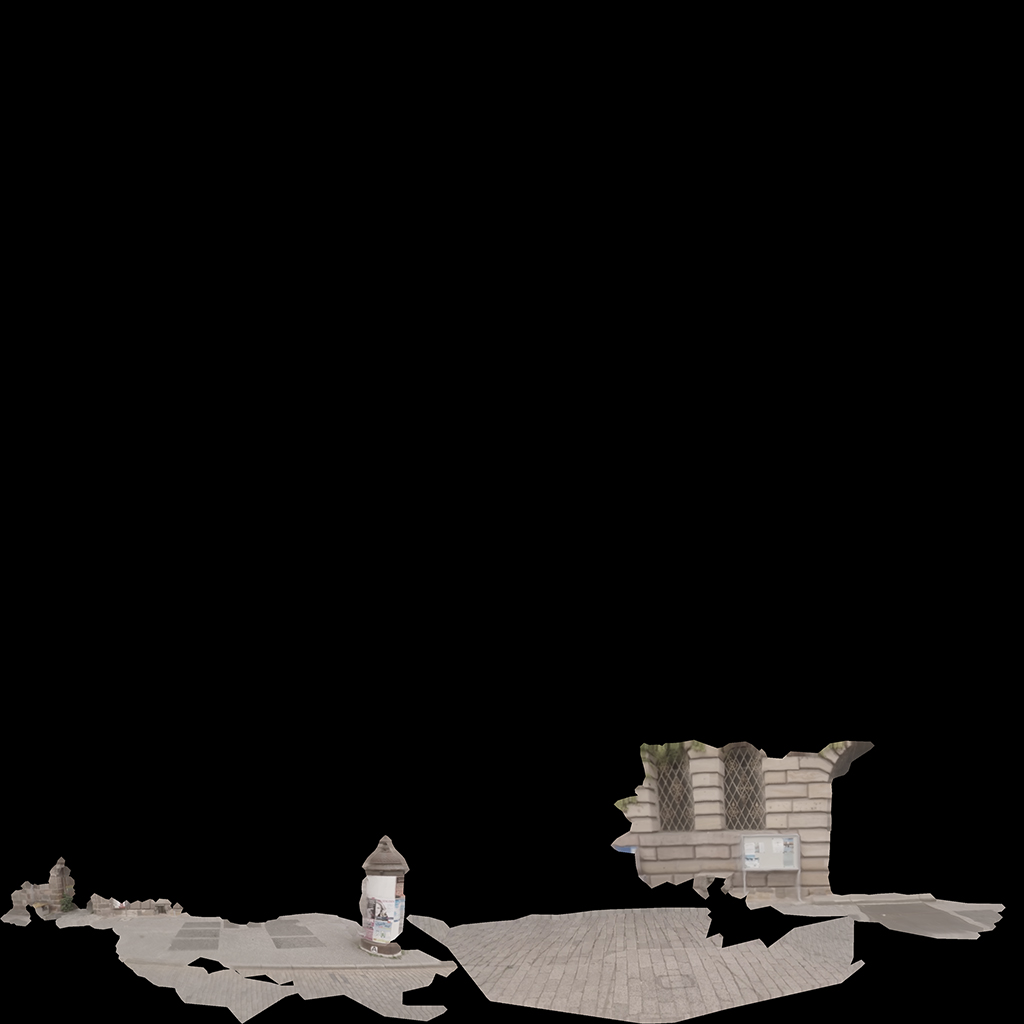
\includegraphics[width=\textwidth]{Delaunay_Tetrahedralization_texture_map_1.jpg}
		\caption{Big UV islands}
		\label{fig:appendix_dt_1}
	\end{subfigure}
	\hfill
	\begin{subfigure}[b]{0.3\textwidth}
		\centering
		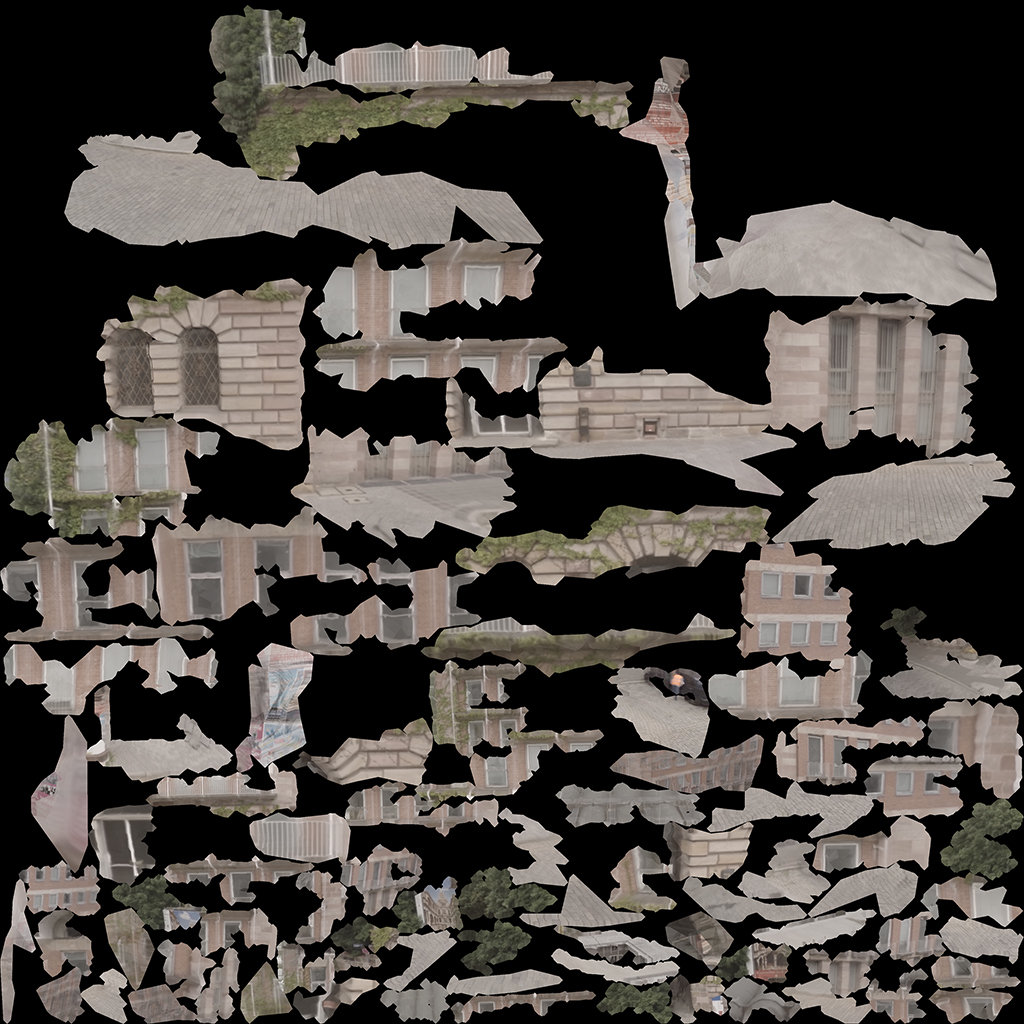
\includegraphics[width=\textwidth]{Delaunay_Tetrahedralization_texture_map_2.jpg}
		\caption{Medium UV islands}
		\label{fig:appendix_dt_2}
	\end{subfigure}
	\hfill
	\begin{subfigure}[b]{0.3\textwidth}
		\centering
		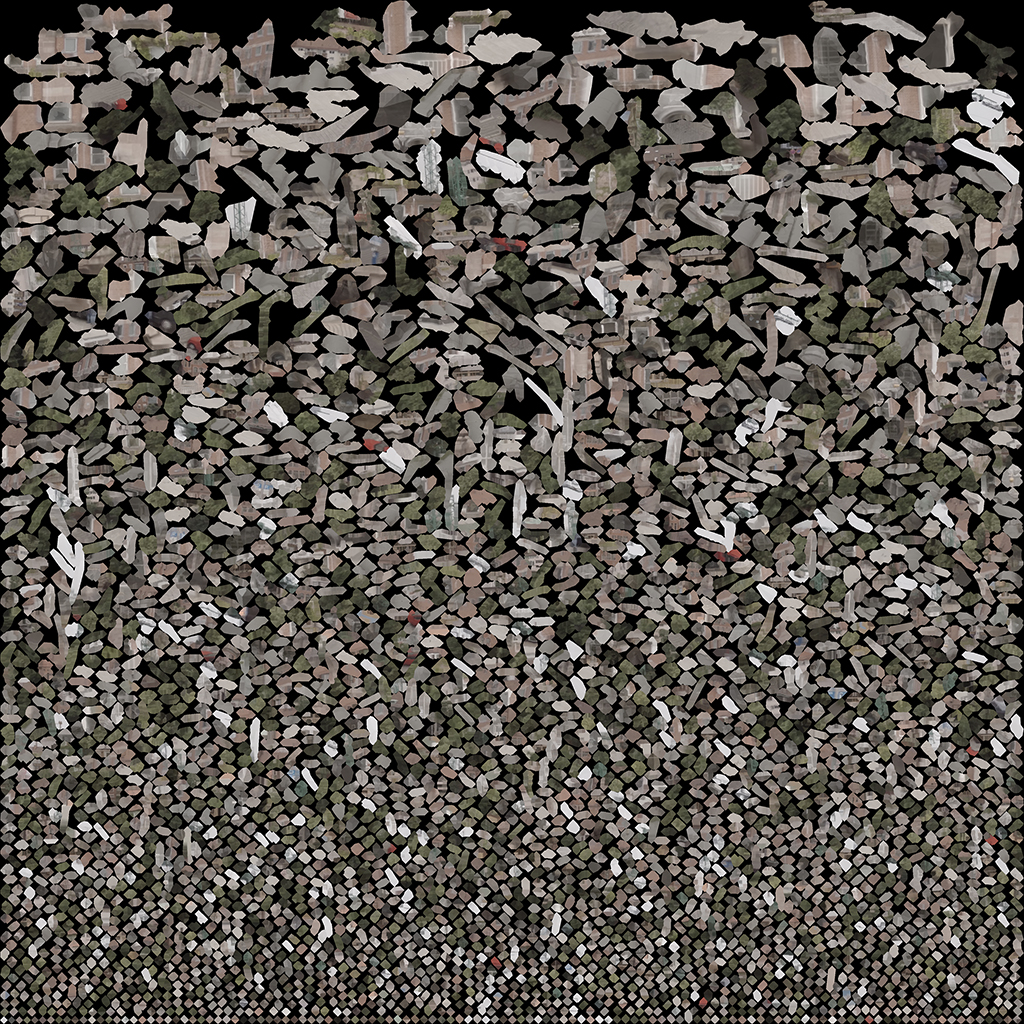
\includegraphics[width=\textwidth]{Delaunay_Tetrahedralization_texture_map_3.jpg}
		\caption{Small UV islands}
		\label{fig:appendix_dt_3}
	\end{subfigure}
	\caption{Texture maps generated with Delaunay Tetrahedralization}
	\label{fig:appendix_dt}
\end{figure}
